\section{Integración Numérica}
\subsection{Motivación}

El objetivo de la integración numérica es aproximar el valor de la integral definida de una función $f$ en un intervalo $[a, b]$ a partir de los valores de la función en ciertos puntos, es decir:
\[
    \begin{array}{c|c}
        x_i & f(x_i) \\
        \hline
        x_0 & f(x_0) \\
        x_1 & f(x_1) \\
        \vdots & \vdots \\
        x_n & f(x_n) \\
    \end{array}
    \longrightarrow
    S = \int_a^b f(x) dx = 
    \underbrace{\widetilde{S}}_{\text{fórmula aproximada}} + \underbrace{E}_{\text{error}}
\]

\subsection{Aproximación por interpolación de Lagrange}

La idea de este procedimiento se va a basar en utilizar los \textbf{Polinomios de Lagrange}:

\[
    \underbrace{f(x)}_{\in C^{n+1}[a,b]} = 
    \underbrace{p_n(x)}_{\text{polinomio de interpolación de Lagrange}} + \underbrace{E_n(x)}_{\text{error de interpolación}}
\]

Dónde:

\[
    p_n(x) = \sum_{i=0}^n f(x_i) L_i(x) \, \qquad L_i(x) = 
    \prod_{\substack{j=0 \\ j \neq i}}^n \frac{x - x_j}{x_i - x_j}
\]
\[
    E_n(x) = \frac{f^{(n+1)}(\xi_x)}{(n+1)!} \prod_{i=0}^n (x - x_i)
\]

De donde se deduce que:
\[
    S = \int_a^b f(x) dx = 
    \underbrace{\int_a^b p_n(x) dx}_{\widetilde{S}_n} + \underbrace{\int_a^b E_n(x) dx}_{E_n}
\]

Ahora podemos escribir la fórmula de aproximación de la integral:
\[
    \widetilde{S}_n = 
    \int_a^b p_n(x) dx = 
    \int_a^b \sum_{i=0}^n f(x_i) L_i(x) dx =
    \sum_{i=0}^n f(x_i) \int_a^b \underbrace{L_i(x)}_{c_i} =
    \boxed{\sum_{i=0}^n c_i f(x_i)}
\]

\subsection{Aproximación por rectángulos}

Es interesante destacar que para calcular integrales existen formulas abiertas, y formulas cerradas. Las fórmulas abiertas no incluyen los extremos del intervalo, mientras que las fórmulas cerradas sí los incluyen.

\begin{center}
    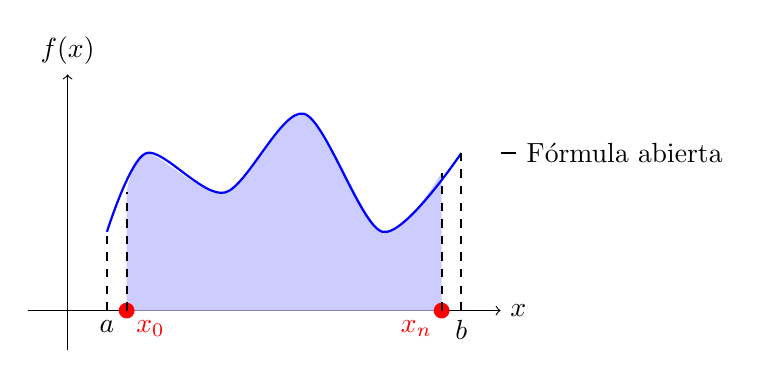
\begin{tikzpicture}
        % Ejes 
        \draw[->] (-0.5, 0) -- (5.5, 0) node[right] {$x$};
        \draw[->] (0, -0.5) -- (0, 3) node[above] {$f(x)$};

        % Area bajo la curva
        \fill[blue!20] (0.75, 0) -- plot[smooth] coordinates {(0.75, 1.5) (1, 2) (2, 1.5) (3, 2.5) (4, 1) (4.75, 1.75)} -- (4.75, 0) -- cycle;

        % Función
        \draw[thick, blue] plot[smooth] coordinates {(0.5, 1) (1, 2) (2, 1.5) (3, 2.5) (4, 1) (5, 2)};

        % Puntos de interpolación x_0 y x_n interiores a [a, b]
        \fill[red] (0.75, 0) circle (0.1) node[below right] {$x_0$};
        \fill[red] (4.75, 0) circle (0.1) node[below left] {$x_n$};

        % Rectas de x_0 y x_n hasta la función
        \draw[thick, dashed] (0.75, 0) -- (0.75, 1.5);
        \draw[thick, dashed] (4.75, 0) -- (4.75, 1.75);

        % Intervalo [a, b]
        \draw[thick, dashed] (0.5, 0) -- (0.5, 1);
        \draw[thick, dashed] (5, 0) -- (5, 2);
        \node[below] at (0.5, 0) {$a$};
        \node[below] at (5, 0) {$b$};

        % Leyenda abierta
        \draw[thick] (5.5, 2) -- (5.7, 2) node[right] {Fórmula abierta};
    \end{tikzpicture}
\end{center}

\begin{center}
    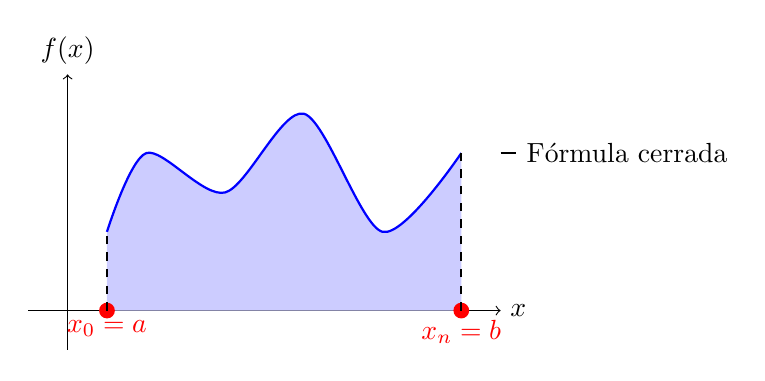
\begin{tikzpicture}
        % Ejes
        \draw[->] (-0.5, 0) -- (5.5, 0) node[right] {$x$};
        \draw[->] (0, -0.5) -- (0, 3) node[above] {$f(x)$};

        % Area bajo la curva
        \fill[blue!20] (0.5, 0) -- plot[smooth] coordinates {(0.5, 1) (1, 2) (2, 1.5) (3, 2.5) (4, 1) (5, 2)} -- (5, 0) -- cycle;

        % Función
        \draw[thick, blue] plot[smooth] coordinates {(0.5, 1) (1, 2) (2, 1.5) (3, 2.5) (4, 1) (5, 2)};

        % Puntos de interpolación x_0 y x_n en los extremos del intervalo
        \fill[red] (0.5, 0) circle (0.1) node[below] {$x_0 = a$};
        \fill[red] (5, 0) circle (0.1) node[below] {$x_n = b$};

        % Rectas de x_0 y x_n hasta la función
        \draw[thick, dashed] (0.5, 0) -- (0.5, 1);
        \draw[thick, dashed] (5, 0) -- (5, 2);

        

        % Leyenda cerrada
        \draw[thick] (5.5, 2) -- (5.7, 2) node[right] {Fórmula cerrada};
    \end{tikzpicture}
\end{center}

Podemos fijar, al igual que en la diferenciación numérica, una distancia fina entre los puntos de interpolación, es decir, $h = \frac{b - a}{n+2}$.

Veamos ahora distintos caos según \textbf{n}.\\

\textbf{Caso $n = 0$:} En este caso, el polinomio de interpolación de Lagrange es simplemente una constante, es decir, $p_0(x) = f(x_0)$. Por lo tanto, la fórmula de aproximación de la integral se reduce a:
\[
    \widetilde{S}_0 = \int_a^b p_0(x) dx = \int_a^b f(x_0) dx = f(x_0)(b - a)
\]

Utilizando ahora que en este caso $h = \frac{b - a}{2}$, podemos escribir la fórmula de aproximación de la integral como:
\[
    \boxed{\widetilde{S}_0 = 2hf(x_0)}
\]

Que es la fórmula del área del rectángulo. Podemos ahora intentar calcular el error cometido usando la siguiente función:
\[
    \begin{array}{cccc}
        \varphi: & [0, h] & \longrightarrow & \mathbb{R} \\
        & x & \longmapsto & \varphi(x)
    \end{array} \longrightarrow
    \varphi(r) = \underbrace{\int_{x_0-r}^{x_0+r} f(x) dx}_{\text{exacto}} - \underbrace{2rf(x_0)}_{\text{aproximación}}
\]

Donde $r \in [0, h]$, y nos deja:
\[
    \varphi(0) = 0, \qquad \varphi(h) = \epsilon_0
\]

Siendo $\epsilon_0$ el error cometido. Ahora podemos derivar $\varphi$:
\[
    \boxed{\varphi'(r) = f(x_0 + r) + f(x_0 - r) - 2f(x_0)} \, \qquad \varphi'(0) = 0
\]

Si derivamos por segunda vez, obtenemos:
\[
    \varphi''(r) = f'(x_0 + r) - f'(x_0 - r) \, \qquad \varphi''(0) = 0
\]

Ahora usando Taylor:
\[
    \begin{cases}
        f'(x_0 + r) = f'(x_0) + f''(\xi_r)r  \qquad \xi_r \in (x_0, x_0 + r) \\
        f'(x_0 - r) = f'(x_0) - f''(\eta_r)r \qquad \eta_r \in (x_0 - r, x_0)
    \end{cases}
    \implies  
    \varphi''(r) = 2r \left( \frac{f''(\xi) + f''(\eta)}{2} \right)
\]

Ahora, aplicando el teorema del valor intermedio (Bolzano para los amigos) sobre $\frac{f''(\xi) + f''(\eta)}{2}$, obtenemos que existe $\theta \in (x_0 - r, x_0 + r)$ tal que:
\[
    \varphi''(r) = 2rf''(\theta)
\]

Ahora podemos integrar $\varphi''$ para obtener:
\[
    \begin{cases}
        \int_0^r \varphi''(s) ds = \varphi'(r) - \varphi'(0) = \varphi'(r) \\
        \int_0^r 2sf''(\theta) ds = f''(\theta) s^2 \Big|_0^r = f''(\theta) r^2
    \end{cases}
    \implies 
    \boxed{\varphi'(r) = f''(\theta) r^2}
\]

Dejando así finalmente las fórmulas para aproximar la integral y el error cometido:
\[
    S = \int_a^b f(x) dx \approx 2hf(x_0)
\]
\[
    E = \varphi(h) = \frac{f''(\theta)}{3} h^3
\]

\subsection{Aproximación por trapecios}

Utilizaremos la fórmula de aproximación de la integral mediante trapecios, dejando de  nuevo la constante $h$. Para el caso $n = 0$, tenemos el siguiente trapecio:
\begin{center}
    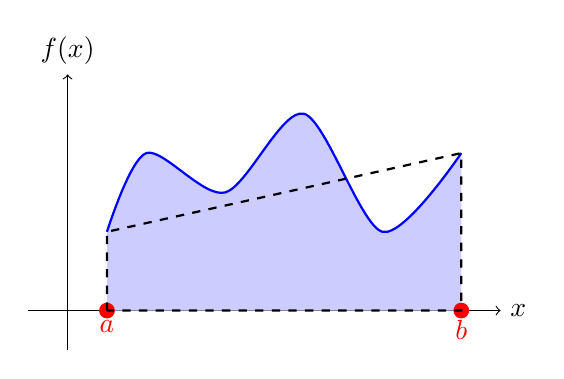
\begin{tikzpicture}
        % Ejes
        \draw[->] (-0.5, 0) -- (5.5, 0) node[right] {$x$};
        \draw[->] (0, -0.5) -- (0, 3) node[above] {$f(x)$};

        % Area bajo la curva
        \fill[blue!20] (0.5, 0) -- plot[smooth] coordinates {(0.5, 1) (1, 2) (2, 1.5) (3, 2.5) (4, 1) (5, 2)} -- (5, 0) -- cycle;

        % Función
        \draw[thick, blue] plot[smooth] coordinates {(0.5, 1) (1, 2) (2, 1.5) (3, 2.5) (4, 1) (5, 2)};

        % Puntos de interpolación a y b
        \fill[red] (0.5, 0) circle (0.1) node[below] {$a$};
        \fill[red] (5, 0) circle (0.1) node[below] {$b$};

        % Trapecio a b f(a) f(b)
        \draw[thick, dashed] (0.5, 0) -- (0.5, 1) -- (5, 2) -- (5, 0) -- cycle;
    \end{tikzpicture}
\end{center}

Donde aproximamos la integral por el área del trapecio, es decir:
\[
    S = \int_a^b f(x) dx \approx (b-a) \frac{f(a) + f(b)}{2} = \frac{h}{2} (f(a) + f(b))
\]

Si vamos con la aproximación por interpolación de Lagrange, tenemos que:
\[
    \widetilde{S} = \int_a^b p_1(x) dx = \sum_{i=0}^1 f(x_i) \underbrace{\int_a^b L_i(x) dx}_{c_i}
\]

Donde ahora si tomamos $x_0 = a$ y $x_1 = b$, obteniendo que:
\[
    \begin{cases}
        L_0(x) = \frac{x - x_1}{x_0 - x_1} = \frac{x - b}{-h} \implies
        c_0 = \int_a^b L_0(x) dx = 
        \int_a^b \frac{b - x}{h} dx =
        - \frac{(x-b)^2}{2h} \Big|_a^b = \boxed{\frac{h}{2}} \\
        L_1(x) = \frac{x - x_0}{x_1 - x_0} = \frac{x - a}{h} \implies
        c_1 = \int_a^b L_1(x) dx =
        \int_a^b \frac{x - a}{h} dx =
        \frac{(x-a)^2}{2h} \Big|_a^b = \boxed{\frac{h}{2}}
    \end{cases}
\]

Y el error en este caso sería:
\[
    E = \int_a^b \underbrace{E_1(x)}_{\text{error de interpolación}} dx =
    \int_a^b \frac{f''(\xi_x)}{2!} (x - a)(x - b) dx
\]

Ahora recordemos el teorema del valor medio para integrales.
\begin{teorema}[Teorema del valor medio para integrales]
    Si $h,g \in C[a,b]$, entonces $\exists \theta \in (a,b)$ tal que:
    \[
        \int_a^b h(x)g(x) dx = h(\theta) \int_a^b g(x) dx
    \]
\end{teorema}

Ahora, podemos continuar tomando:
\[
    E = \int_a^b \underbrace{\frac{f''(\xi_x)}{2}}_{h(x)} \underbrace{(x - a)(x - b)}_{g(x)} dx =
    \frac{f''(\theta)}{2} \int_a^b (x - a)(x - b) dx =
    \frac{f''(\theta)}{2} - \frac{h^3}{6} =
    -\frac{f''(\theta)}{12} h^3
\]

Resumiendo, nos quedan los siguientes errores según el método utilizado, y recordando que en el rectángulo $h = \frac{b - a}{2}$, mientras que en el trapecio $h = b - a$:
\[
    E_{\text{rectángulos}} = \frac{f''(\theta)}{3} h_R^3 = \frac{f''(\theta)}{24} h^3
\]
\[
    E_{\text{trapecios}} = -\frac{f''(\theta)}{12} h_T^3 = -\frac{f''(\theta)}{12} h^3
\]

Donde se aprecia que el error cometido por el método de los trapecios es el doble que el error cometido por el método de los rectángulos. Por lo tanto, el método de los rectángulos es más preciso que el método de los trapecios.\\

Algo interesante a notar en este caso es que si la 2 derivada es 0, ocurre lo siguiente:
\[
    f''(\theta) = 0 \implies
    \begin{cases}
        E_{\text{rectángulos}} = 0 \\
        E_{\text{trapecios}} = 0
    \end{cases}
\]

También es interesante destacar que normalmente las fórmulas abiertas son más precisas que las cerradas.

\subsection{Formula del trapecio abierta}

Si tomamos $n = 0$, pero ahora con $x_0$ y $x_1$ interiores a $[a, b]$, con $h=\frac{b - a}{3}$, tenemos la siguiente aproximación de la integral:
\begin{center}
    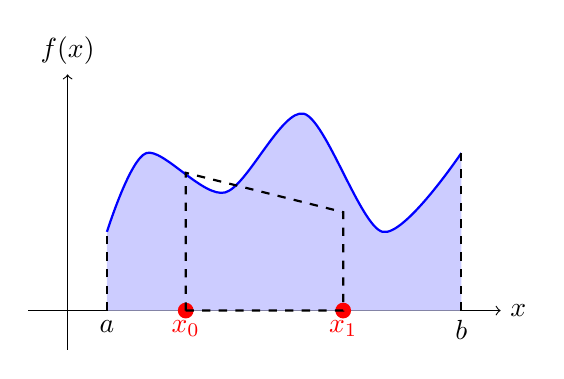
\begin{tikzpicture}
        % Ejes
        \draw[->] (-0.5, 0) -- (5.5, 0) node[right] {$x$};
        \draw[->] (0, -0.5) -- (0, 3) node[above] {$f(x)$};

        % Area bajo la curva
        \fill[blue!20] (0.5, 0) -- plot[smooth] coordinates {(0.5, 1) (1, 2) (2, 1.5) (3, 2.5) (4, 1) (5, 2)} -- (5, 0) -- cycle;
        % Función
        \draw[thick, blue] plot[smooth] coordinates {(0.5, 1) (1, 2) (2, 1.5) (3, 2.5) (4, 1) (5, 2)};

        % Puntos de interpolación x_0 y x_1 interiores a [a, b]
        \fill[red] (1.5, 0) circle (0.1) node[below] {$x_0$};
        \fill[red] (3.5, 0) circle (0.1) node[below] {$x_1$};

        % Trapecio x_0 x_1 f(x_0) f(x_1)
        \draw[thick, dashed] (1.5, 0) -- (1.5, 1.75) -- (3.5, 1.25) -- (3.5, 0) -- cycle;

        % Marcas a y b
        \draw[thick, dashed] (0.5, 0) -- (0.5, 1);
        \draw[thick, dashed] (5, 0) -- (5, 2);
        \node[below] at (0.5, 0) {$a$};
        \node[below] at (5, 0) {$b$};

    \end{tikzpicture}
\end{center}

El cual nos deja la siguiente fórmula de aproximación de la integral:
\[
    \widetilde{S} = 3h \frac{f(x_0) + f(x_1)}{2}
\]

Con error:
\[
    E = \frac{3}{4} f''(\theta) h^3
\]